\newpage
\begin{appendices}
\section{Lexique}
\begin{itemize}
	\item Protocole réseau :
    Un protocole est une méthode standard qui permet la communication entre des processus (s'exécutant éventuellement sur différentes machines), 
    c'est-à-dire un ensemble de règles et de procédures à respecter pour émettre et recevoir des données sur un réseau. 
    Il en existe plusieurs selon ce que l'on attend de la communication. Certains protocoles seront par exemple spécialisés dans l'échange de fichiers (le FTP), 
    d'autres pourront servir à gérer simplement l'état de la transmission et des erreurs (c'est le cas du protocole ICMP), ... 
\newline

	\item TCP : 
    Acronyme de Transmission Control Protocol, le protocole TCP/IP est le protocole standard utilsié sur internet, pour la liaison entre deux ordinateurs.
    Le protocoel TCP vérifie la validité des paquets après leur réception afin d'être sur de la validité de celle-ci. 
    Le protocole TCP est située sur la couche 4 (couche de transport) du modèle OSI. 
\newline

	\item UDP :
    Acronyme User Datagram Protocol, le protocole UDP est un des protocoles standards utilisé sur internet. 
    La différence avec TCP est que les paquets sont reçus sous forme de datagramme qui doit être vérifier pour valider la qualité du paquet reçu.
    Le protocole UDP est très utilisé, notamment, dans le cadre du jeu en ligne, ou encore le streaming, car la perte de paquet influe peu sur la quantité reçus.
    Le protocole UDP est située sur la couche 4 (couche de transport) du modèle OSI, au même titre que le protocole TCP. 
   \newline
 
	\item Socket :
    Une socket est une interface de connexion bidirectionnelle permettant l'échange de données entre deux processus (distants ou non).
   \newline
 
	\item Socket de Berkeley :
    Les sockets de Berkeley, sont un ensemble normalisés de fonctions de communications lancé par l'université de Berkeley au début des années 1980.
    De nos jours, elle est la norme utilisé par quasiment l'ensemble des langages de développement (C, Java, Python, ...).
  \newline
  
	\item Pair à  pair :
    Le pair à  pair (ou peer-to-peer en anglais), est un modèle de réseau permettant à  deux machines de discuter d'égale à  égale.
    Dans les faits, cela s'explique par le fait qu'une machine se connecte a une autre machine et inversement afin que celles-ci puissent s'échanger des informations
    sans passer par un serveur distant.
\end{itemize}


\newpage
\section{Webographie}
\begin{itemize}
	\item Fonctionnement des intelligences artificielles : \url{http://www.datagenetics.com/blog/december32011/index.html}
\newline	
	\item API Java : \url{https://docs.oracle.com/javase/7/docs/api/}
	\newline
	\item Règles de la bataille navale: \url{http://www.regles-de-jeux.com/regle-de-la-bataille-navale/}
\end{itemize}

\newpage
\section{Schéma du protocole de l'application}
\begin{sidewaysfigure}
    \centering
    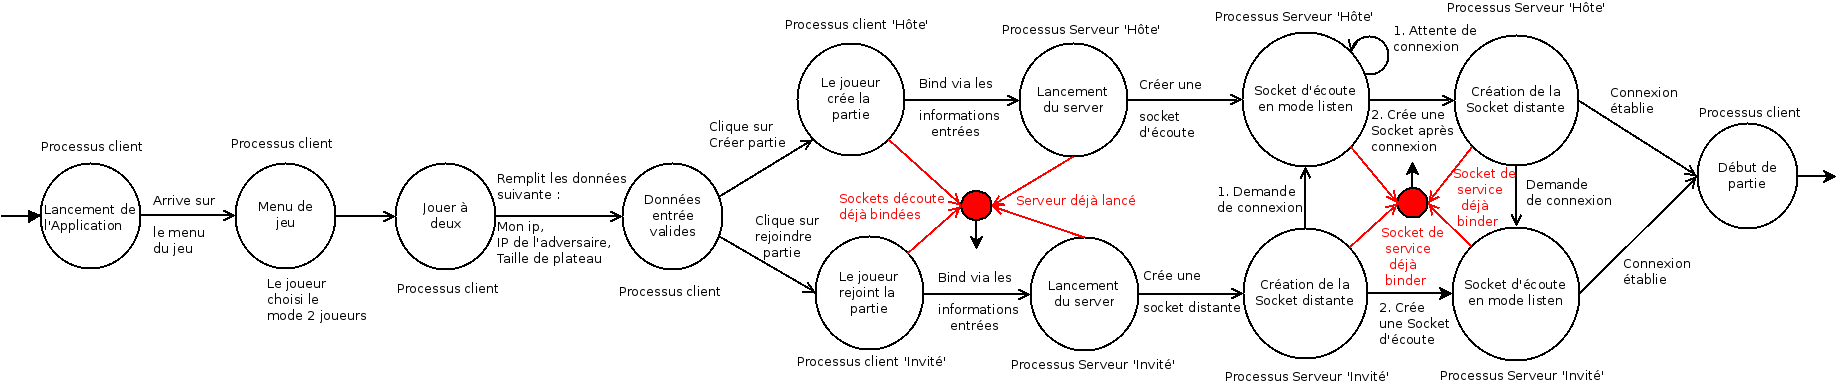
\includegraphics [width=215mm]{images/connection_between_players.png}
    \caption{Schéma représetant le protocole de connexion entre deux joueurs}
    \label{connection}
\end{sidewaysfigure}
\begin{sidewaysfigure}
    \centering
    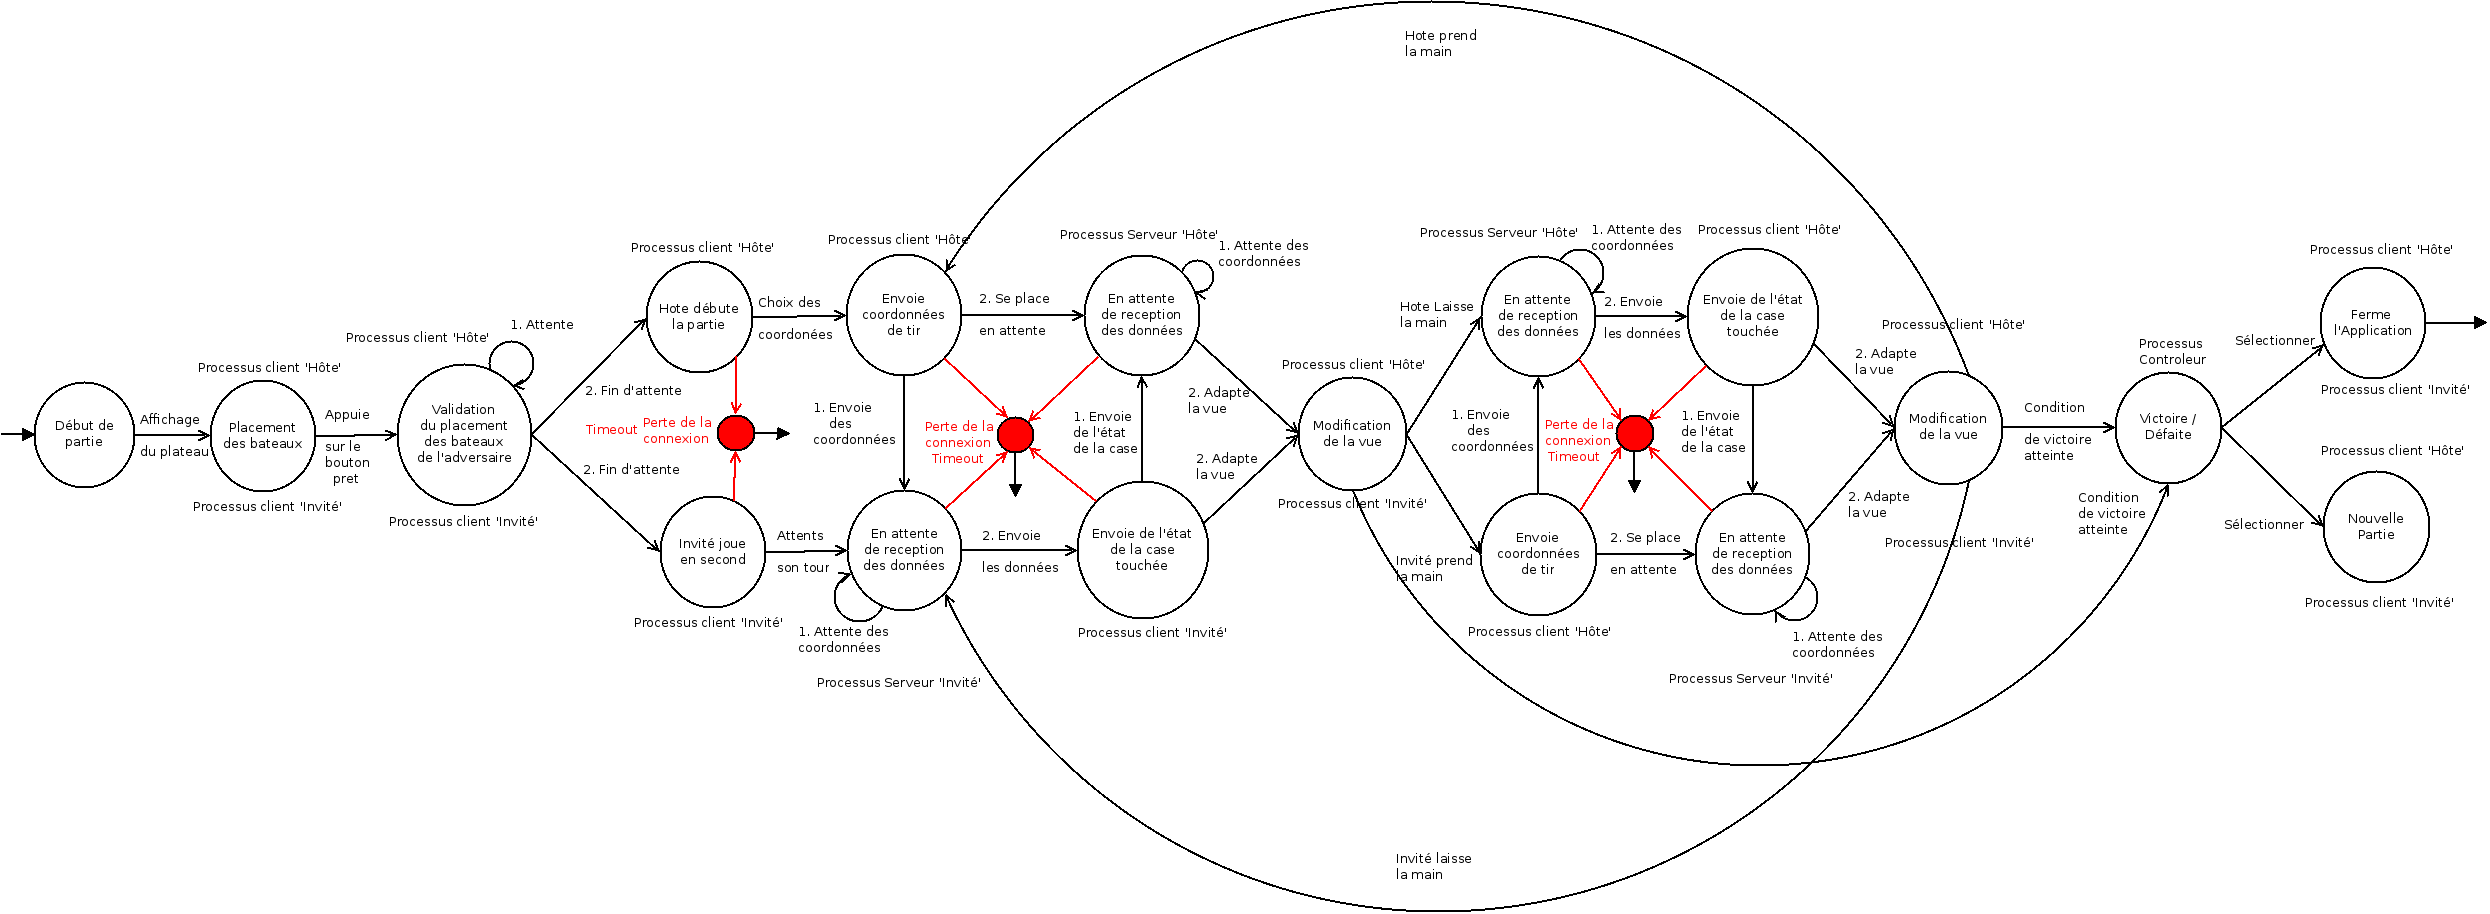
\includegraphics [width=215mm]{images/data_exhange_between_players.png}
    \caption{Schéma représetant le protocole d'échange de données entre deux joueurs}
    \label{connection}
\end{sidewaysfigure}

\end{appendices}